\chapter{Solution proposal}\label{cha:solution}

This chapter is intended to give the reader a summary of the proposed solution and its structure, as well as 
the technical specifications that were given and taken into account. Any other constraint not mentioned here 
was adjusted or set while being within the design-test loop, as consequence of the prototype nature of the project.

\section{Technical specifications}

In table \ref{tbl:tech_specs} the requirements for this prototype and their state after the implementation can be observed.
This comparison helps as a good summary of the overall achievments that are further detailed in the next sections.

  \begin{tuhhtable}
    \footnotesize\centering
    \begin{tabular}[tp]{L{.22\textwidth}L{.22\textwidth}L{.22\textwidth}L{.22\textwidth}}
        \THc{1}{c}{Feature} & \THc{1}{c}{Requirement} & \THc{1}{c}{Implementation} & \THc{1}{c}{Remark} \\
      \abovebodyrule
      \TRh{1}{l}{Upper layer interface}  & Ethernet/EtherCAT compatibility.\newline Non-safety relevant.\newline Services and synchronization: tbd 
                                        & EtherCAT slave.\newline Services: Mailboxing and CoE\newline Synchronization: Free Run and SM  
                                        & \tblYes\newline FoE and SD synchronization possible in the medium term.\\\TRc
      \TRhc{1}{l}{Display/signaling}    & LED stripes with serial interface:\newline WS2812 \newline 2 Ch  
                                        & 2-4 Ch modifiable in SW\newline Animation capable 
                                        & \tblYes\newline Chs can increase up to number of DMA-Timers (8*)   \\
      \TRh{1}{l}{Temperature}           & Data interface for 1-Wire bus     
                                        & 1-Wire Master\newline 15 sensor in bus & \tblYes\newline 6 Sensors simultaneously tested \\\TRc
      \TRhc{1}{l}{PCB}                  & PCB Prototype\newline Layout and size: tbd   
                                        & Attachable PCB for LAN9252-EVB-SPI.\newline Size: 55mm$x$38mm & \tblYes\newline Second layout with both chips included posible in the short term. \\
      \TRh{1}{l}{Safety}                & \tblNA     
                                        & Non-safety relevant for this prototype & \tblNo\newline SFoE could be researched in the long term.\\\TRc
      \TRhc{1}{l}{Extra interface}      & SPI or I2C interface for current/IMU/black channel   
                                        & Extra SPI considered in PCB and SW\newline JTAG/SWD compatible interface & \tblYes   \\
      \TRh{1}{l}{Speed/position}        & Possible interface of BISS-C type
                                        & Not required for this prototype & \tblNo \\\TRc
      \TRhc{1}{l}{Refresh data cycle}   & tbd   
                                        & No hard RT deadlines.\newline Deterministic refresh cycle of \texttildelow 10ms by RTOS.\newline Timeout faults handling. & \tblGood   \\
      \TRh{1}{l}{Data structure}        & tbd     
                                        & Functional and parametrization data structure as Object Dictionary.\newline Standard ESI file. & \tblYes \\\TRc
      \TRhc{1}{l}{FW programming}       & \tblNA   
                                        & CMSIS - FreeRTOS for thread, event and time management. & \tblGood   \\
      \belowbodyrule
    \end{tabular}
    \caption{Technical specifications}
    \label{tbl:tech_specs}
  \end{tuhhtable}

\section{Available Hardware}

In this part it is presented the base hardware that was available to develop the prototype. The microcontroller (MCU) was chosen
due to its active community, resources and current on-develop projects. Other MCUs were considered since the overall characteristics
are somewhat similar and generic -regarding peripherals like serial interfaces or dma, processing power and memory, for instance-. 
MCUs from Infineon \cite{infineon_esc}\cite{infineon_dramfine} and 
Texas Instruments \cite{texasi_esc} were good possible candidates; however, the basic familiarity with the STM32CUBE IDE and the related ST technology 
was a crucial factor, since the learning curve is not negligible when it comes to develop any firmware at a fair level, even more when it deals with other to-learn*
technologies, for instance, development with RTOS, modification of open libraries, EtherCAT protocol and the Network Controller chip.

Regarding the Network Controller, the LAN9252 belongs to a set of ASICs that are verified and certified by Beckhoff GmbH. For a further
reference for other alternatives visit \cite{beckhoff_esccomparison}. The LAN9252 integrates a so-called EtherCAT Slave Controller (ESC) and it represents a good 
alternative to the Beckhoff's original ASIC ET1100. This way, the basic hardware is there to fulfill \emph{Han's Robot Germany}'s
proposal for developing industrial compatible devices that could enhance the prototyping process within the electronics department. 
Moreover, the mentioned ASIC has a wide compatible control interface that make it be suitable to any microcontroller with which 
the developer has experience. The table \ref{tbl:hardware_characteristics} lists main characteristics of the above mentioned hardware.

\begin{tuhhtable}
    \footnotesize\centering
    \begin{tabular}[tp]{L{.44\textwidth}L{.44\textwidth}}
        \THc{1}{c}{STM32F446ZE} & \THc{1}{c}{LAN9252} \\
      \abovebodyrule
        ARM®32-bit Cortex®-M4 + FPU + Chrom-ART™ Accelerator
        Up to 180MHz CPU\newline
        512 kB of Flash\newline
        128 KB of SRAM
                                        & EtherCAT slave controller with
                                        3 FMMUs and 4 SyncManagers\newline
                                        Distributed clock support\newline
                                        4KB of DPRAM\\\TRc
        General-purpose DMA\newline
        Up to 17 timers\newline
        Up to 4 × I2 C interfaces\newline
        Up to 4 USARTs/2 UARTs\newline
        Up to 4 SPIs\newline
        2 × CAN (2.0B Active)\newline
        USB 2.0 full-speed device/host/OTG 
                                        &100Mbps Ethernet transceivers compliant with IEEE 802.3/802.3u (Fast Ethernet)\newline
                                        8/16-Bit Host Bus Interface, indexed register or multiplexed bus\newline
                                        SPI/Quad SPI\newline
                                        Digital I/O Mode\newline
                                        Multifunction GPIOs
                                        \\
        LQFP64, LQFP100 and LQFP144 packaging     
                                        & Pb-free RoHS compliant 64-pin QFN or 64-pin TQFPEP packaging 
                                        \\\TRc
      \belowbodyrule
    \end{tabular}
    \caption{Summary of the characteristics of both STM32F446ZE and LAN9252 used in the prototype.}
    \label{tbl:hardware_characteristics}
  \end{tuhhtable}

%\subfigbox{
%    \subfigure[NUCLEO-STM32F446ZE]{\label{subfig:stmboard}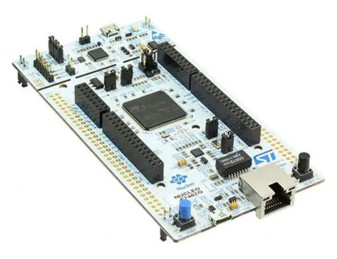
\includegraphics{imgs/sol-stmboard.jpg}}
%    \subfigure[LAN9252-EVB-SPI]{\label{subfig:lanboard}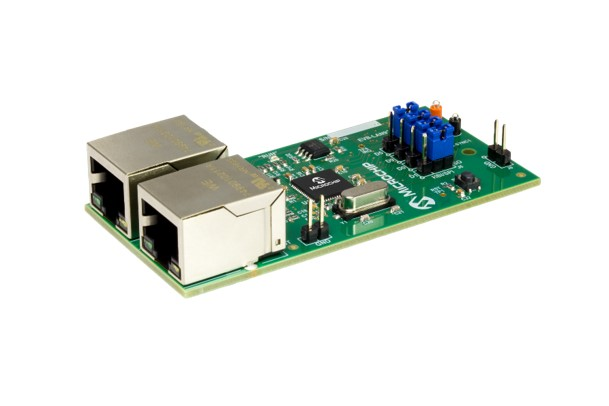
\includegraphics{imgs/sol-lanboard.jpg}}
%}{Evaluation boards for prototyping.}{fig:evalboards}

\begin{figure}[ht]
    \centering
    \subfigure[NUCLEO-STM32F446ZE]{\label{subfig:stmboard}{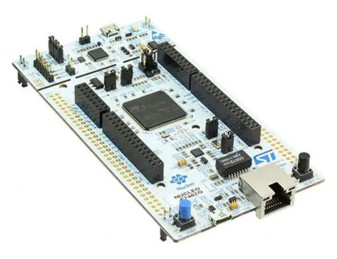
\includegraphics[width=0.4\textwidth]{imgs/sol-stmboard.jpg}}}\hfill
    \subfigure[LAN9252-EVB-SPI]{\label{subfig:lanboard}{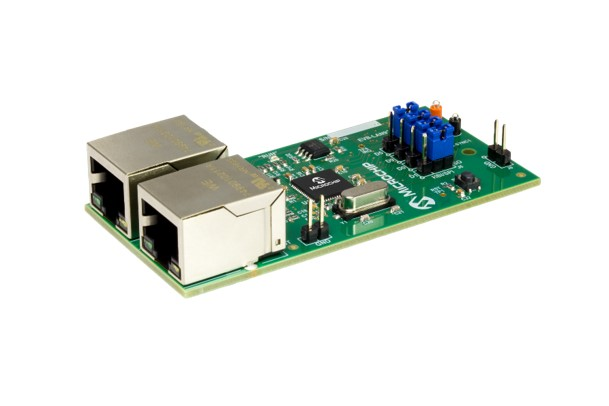
\includegraphics[width=0.4\textwidth]{imgs/sol-lanboard.jpg}}}
    \caption{Evaluation boards for prototyping.}
    \label{fig:evalboards}
\end{figure}

\section{PCB proposal}
As it can be seen in the Fig. \ref{subfig:lanboard}, the evaluation board counts with on-board male pins, this was taken as an advantage and the PCB to be designed
consisted on a plugable PCB that would be mounted on top of it, increasing minimaly the volume already occupied by the evaluation board. This idea needed to be 
designed taking into account the minimum of components based on the Nucleo-STM32F446ZE original design and the requirements of the LAN9252. This means that 
it had to provide, both 5V and 3.3 V power supply, physical ports for the prioritized communication capabilities, minimaly SPI, One-Wire JTAG and the LED ports 
according to the technical specifications \ref{tbl:tech_specs}.

\section{Software structure}
The final proposal for the structure of the embedded system can be seen in fig. ~\ref{fig:sysStruct}. 
The functional blocks represented in grey or dashed lines are mainly components that are planned not to be modified
at all or not in deep, because of either its complexity or its given reliability. This means its functionality is almost granted. 
Nevertheless, the progress relies on documentation that can be either good or poor, for instance, TwinCAT has good resources, 
whereas SOES does not. 
Another thing to keep in mind is the abreviation DSM (Device's State Machine) which is used in this document as substitute for State Machine,
such that it is not confused with Synchronization Manager, defined as well by Beckhoff as SM.
\begin{figure}[ht]
    \centering
    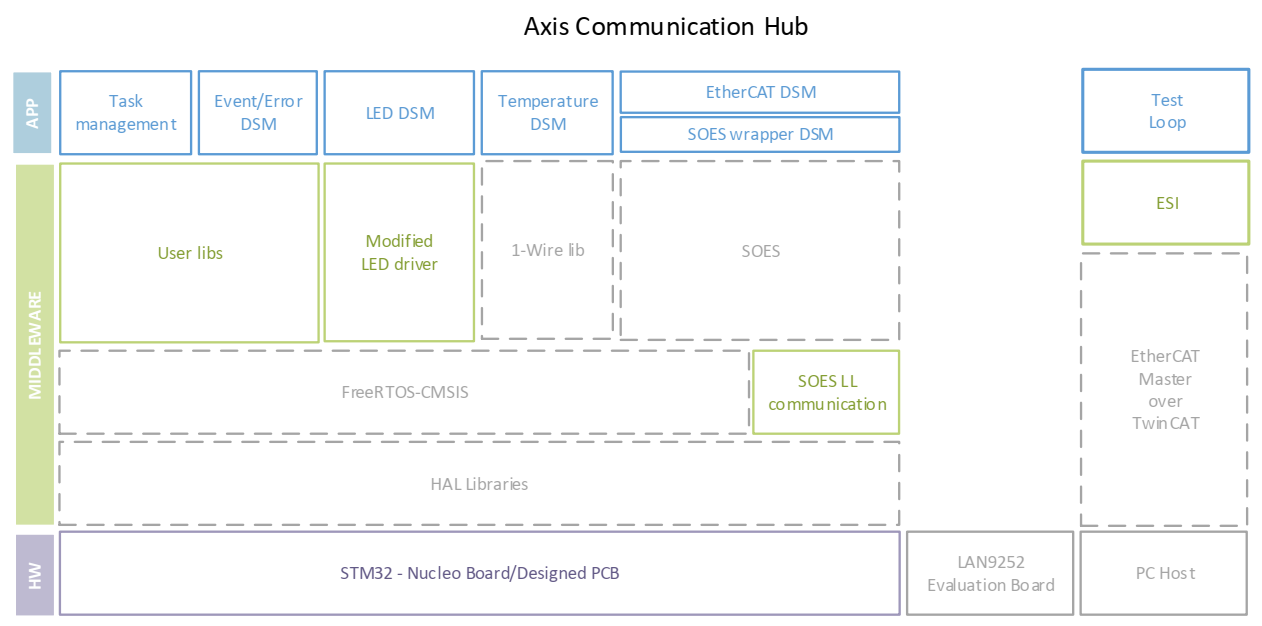
\includegraphics[width=\textwidth]{imgs/prop-system_struct_v2.png}
    \caption{Layered strcuture of the proposed functional blocks.}
    \label{fig:sysStruct}
\end{figure}



%TODO this figure needs to be updated changing the Error handler to Event handler, configuration/management to auxiliar functions --monitor for debugging
%adding as well the ESI file as a functional block running on top of the LAN9252 Evaluation board
%Where could I mention about the wrappers used to integrate the functions contained within the 3rd party libraries and my SMS?